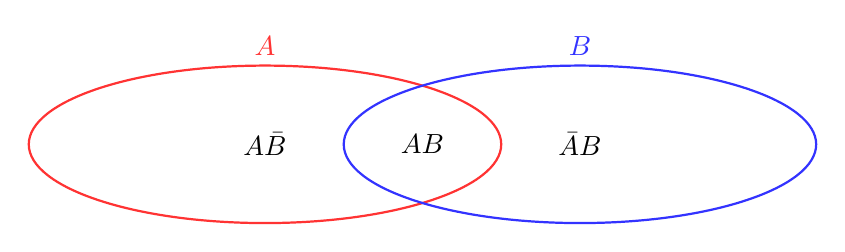
\begin{tikzpicture}

  \draw[color = red!80] (-2, 1) node[above] {\(A\)};
  \draw[thick, color = red!80] (-2, 0) ellipse (3 and 1);

  \draw[color = blue!80] (2, 1) node[above] {\(B\)};
  \draw[thick, color = blue!80] (2, 0) ellipse (3 and 1);

  \draw (-2, 0) node {\(A \bar{B}\)};
  \draw (0, 0) node {\(A B\)};
  \draw (2, 0) node {\(\bar{A} B\)};
  
\end{tikzpicture}